\documentclass{article}
\PassOptionsToPackage{table}{xcolor} % eso-pic in the official style loads xcolor first
\usepackage{iclr2027_conference,times}
%%%%% NEW MATH DEFINITIONS %%%%%

\usepackage{amsmath,amsfonts,bm}

% Mark sections of captions for referring to divisions of figures
\newcommand{\figleft}{{\em (Left)}}
\newcommand{\figcenter}{{\em (Center)}}
\newcommand{\figright}{{\em (Right)}}
\newcommand{\figtop}{{\em (Top)}}
\newcommand{\figbottom}{{\em (Bottom)}}
\newcommand{\captiona}{{\em (a)}}
\newcommand{\captionb}{{\em (b)}}
\newcommand{\captionc}{{\em (c)}}
\newcommand{\captiond}{{\em (d)}}

% Highlight a newly defined term
\newcommand{\newterm}[1]{{\bf #1}}


% Figure reference, lower-case.
\def\figref#1{figure~\ref{#1}}
% Figure reference, capital. For start of sentence
\def\Figref#1{Figure~\ref{#1}}
\def\twofigref#1#2{figures \ref{#1} and \ref{#2}}
\def\quadfigref#1#2#3#4{figures \ref{#1}, \ref{#2}, \ref{#3} and \ref{#4}}
% Section reference, lower-case.
\def\secref#1{section~\ref{#1}}
% Section reference, capital.
\def\Secref#1{Section~\ref{#1}}
% Reference to two sections.
\def\twosecrefs#1#2{sections \ref{#1} and \ref{#2}}
% Reference to three sections.
\def\secrefs#1#2#3{sections \ref{#1}, \ref{#2} and \ref{#3}}
% Reference to an equation, lower-case.
\def\eqref#1{equation~\ref{#1}}
% Reference to an equation, upper case
\def\Eqref#1{Equation~\ref{#1}}
% A raw reference to an equation---avoid using if possible
\def\plaineqref#1{\ref{#1}}
% Reference to a chapter, lower-case.
\def\chapref#1{chapter~\ref{#1}}
% Reference to an equation, upper case.
\def\Chapref#1{Chapter~\ref{#1}}
% Reference to a range of chapters
\def\rangechapref#1#2{chapters\ref{#1}--\ref{#2}}
% Reference to an algorithm, lower-case.
\def\algref#1{algorithm~\ref{#1}}
% Reference to an algorithm, upper case.
\def\Algref#1{Algorithm~\ref{#1}}
\def\twoalgref#1#2{algorithms \ref{#1} and \ref{#2}}
\def\Twoalgref#1#2{Algorithms \ref{#1} and \ref{#2}}
% Reference to a part, lower case
\def\partref#1{part~\ref{#1}}
% Reference to a part, upper case
\def\Partref#1{Part~\ref{#1}}
\def\twopartref#1#2{parts \ref{#1} and \ref{#2}}

\def\ceil#1{\lceil #1 \rceil}
\def\floor#1{\lfloor #1 \rfloor}
\def\1{\bm{1}}
\newcommand{\train}{\mathcal{D}}
\newcommand{\valid}{\mathcal{D_{\mathrm{valid}}}}
\newcommand{\test}{\mathcal{D_{\mathrm{test}}}}

\def\eps{{\epsilon}}


% Random variables
\def\reta{{\textnormal{$\eta$}}}
\def\ra{{\textnormal{a}}}
\def\rb{{\textnormal{b}}}
\def\rc{{\textnormal{c}}}
\def\rd{{\textnormal{d}}}
\def\re{{\textnormal{e}}}
\def\rf{{\textnormal{f}}}
\def\rg{{\textnormal{g}}}
\def\rh{{\textnormal{h}}}
\def\ri{{\textnormal{i}}}
\def\rj{{\textnormal{j}}}
\def\rk{{\textnormal{k}}}
\def\rl{{\textnormal{l}}}
% rm is already a command, just don't name any random variables m
\def\rn{{\textnormal{n}}}
\def\ro{{\textnormal{o}}}
\def\rp{{\textnormal{p}}}
\def\rq{{\textnormal{q}}}
\def\rr{{\textnormal{r}}}
\def\rs{{\textnormal{s}}}
\def\rt{{\textnormal{t}}}
\def\ru{{\textnormal{u}}}
\def\rv{{\textnormal{v}}}
\def\rw{{\textnormal{w}}}
\def\rx{{\textnormal{x}}}
\def\ry{{\textnormal{y}}}
\def\rz{{\textnormal{z}}}

% Random vectors
\def\rvepsilon{{\mathbf{\epsilon}}}
\def\rvtheta{{\mathbf{\theta}}}
\def\rva{{\mathbf{a}}}
\def\rvb{{\mathbf{b}}}
\def\rvc{{\mathbf{c}}}
\def\rvd{{\mathbf{d}}}
\def\rve{{\mathbf{e}}}
\def\rvf{{\mathbf{f}}}
\def\rvg{{\mathbf{g}}}
\def\rvh{{\mathbf{h}}}
\def\rvu{{\mathbf{i}}}
\def\rvj{{\mathbf{j}}}
\def\rvk{{\mathbf{k}}}
\def\rvl{{\mathbf{l}}}
\def\rvm{{\mathbf{m}}}
\def\rvn{{\mathbf{n}}}
\def\rvo{{\mathbf{o}}}
\def\rvp{{\mathbf{p}}}
\def\rvq{{\mathbf{q}}}
\def\rvr{{\mathbf{r}}}
\def\rvs{{\mathbf{s}}}
\def\rvt{{\mathbf{t}}}
\def\rvu{{\mathbf{u}}}
\def\rvv{{\mathbf{v}}}
\def\rvw{{\mathbf{w}}}
\def\rvx{{\mathbf{x}}}
\def\rvy{{\mathbf{y}}}
\def\rvz{{\mathbf{z}}}

% Elements of random vectors
\def\erva{{\textnormal{a}}}
\def\ervb{{\textnormal{b}}}
\def\ervc{{\textnormal{c}}}
\def\ervd{{\textnormal{d}}}
\def\erve{{\textnormal{e}}}
\def\ervf{{\textnormal{f}}}
\def\ervg{{\textnormal{g}}}
\def\ervh{{\textnormal{h}}}
\def\ervi{{\textnormal{i}}}
\def\ervj{{\textnormal{j}}}
\def\ervk{{\textnormal{k}}}
\def\ervl{{\textnormal{l}}}
\def\ervm{{\textnormal{m}}}
\def\ervn{{\textnormal{n}}}
\def\ervo{{\textnormal{o}}}
\def\ervp{{\textnormal{p}}}
\def\ervq{{\textnormal{q}}}
\def\ervr{{\textnormal{r}}}
\def\ervs{{\textnormal{s}}}
\def\ervt{{\textnormal{t}}}
\def\ervu{{\textnormal{u}}}
\def\ervv{{\textnormal{v}}}
\def\ervw{{\textnormal{w}}}
\def\ervx{{\textnormal{x}}}
\def\ervy{{\textnormal{y}}}
\def\ervz{{\textnormal{z}}}

% Random matrices
\def\rmA{{\mathbf{A}}}
\def\rmB{{\mathbf{B}}}
\def\rmC{{\mathbf{C}}}
\def\rmD{{\mathbf{D}}}
\def\rmE{{\mathbf{E}}}
\def\rmF{{\mathbf{F}}}
\def\rmG{{\mathbf{G}}}
\def\rmH{{\mathbf{H}}}
\def\rmI{{\mathbf{I}}}
\def\rmJ{{\mathbf{J}}}
\def\rmK{{\mathbf{K}}}
\def\rmL{{\mathbf{L}}}
\def\rmM{{\mathbf{M}}}
\def\rmN{{\mathbf{N}}}
\def\rmO{{\mathbf{O}}}
\def\rmP{{\mathbf{P}}}
\def\rmQ{{\mathbf{Q}}}
\def\rmR{{\mathbf{R}}}
\def\rmS{{\mathbf{S}}}
\def\rmT{{\mathbf{T}}}
\def\rmU{{\mathbf{U}}}
\def\rmV{{\mathbf{V}}}
\def\rmW{{\mathbf{W}}}
\def\rmX{{\mathbf{X}}}
\def\rmY{{\mathbf{Y}}}
\def\rmZ{{\mathbf{Z}}}

% Elements of random matrices
\def\ermA{{\textnormal{A}}}
\def\ermB{{\textnormal{B}}}
\def\ermC{{\textnormal{C}}}
\def\ermD{{\textnormal{D}}}
\def\ermE{{\textnormal{E}}}
\def\ermF{{\textnormal{F}}}
\def\ermG{{\textnormal{G}}}
\def\ermH{{\textnormal{H}}}
\def\ermI{{\textnormal{I}}}
\def\ermJ{{\textnormal{J}}}
\def\ermK{{\textnormal{K}}}
\def\ermL{{\textnormal{L}}}
\def\ermM{{\textnormal{M}}}
\def\ermN{{\textnormal{N}}}
\def\ermO{{\textnormal{O}}}
\def\ermP{{\textnormal{P}}}
\def\ermQ{{\textnormal{Q}}}
\def\ermR{{\textnormal{R}}}
\def\ermS{{\textnormal{S}}}
\def\ermT{{\textnormal{T}}}
\def\ermU{{\textnormal{U}}}
\def\ermV{{\textnormal{V}}}
\def\ermW{{\textnormal{W}}}
\def\ermX{{\textnormal{X}}}
\def\ermY{{\textnormal{Y}}}
\def\ermZ{{\textnormal{Z}}}

% Vectors
\def\vzero{{\bm{0}}}
\def\vone{{\bm{1}}}
\def\vmu{{\bm{\mu}}}
\def\vtheta{{\bm{\theta}}}
\def\va{{\bm{a}}}
\def\vb{{\bm{b}}}
\def\vc{{\bm{c}}}
\def\vd{{\bm{d}}}
\def\ve{{\bm{e}}}
\def\vf{{\bm{f}}}
\def\vg{{\bm{g}}}
\def\vh{{\bm{h}}}
\def\vi{{\bm{i}}}
\def\vj{{\bm{j}}}
\def\vk{{\bm{k}}}
\def\vl{{\bm{l}}}
\def\vm{{\bm{m}}}
\def\vn{{\bm{n}}}
\def\vo{{\bm{o}}}
\def\vp{{\bm{p}}}
\def\vq{{\bm{q}}}
\def\vr{{\bm{r}}}
\def\vs{{\bm{s}}}
\def\vt{{\bm{t}}}
\def\vu{{\bm{u}}}
\def\vv{{\bm{v}}}
\def\vw{{\bm{w}}}
\def\vx{{\bm{x}}}
\def\vy{{\bm{y}}}
\def\vz{{\bm{z}}}

% Elements of vectors
\def\evalpha{{\alpha}}
\def\evbeta{{\beta}}
\def\evepsilon{{\epsilon}}
\def\evlambda{{\lambda}}
\def\evomega{{\omega}}
\def\evmu{{\mu}}
\def\evpsi{{\psi}}
\def\evsigma{{\sigma}}
\def\evtheta{{\theta}}
\def\eva{{a}}
\def\evb{{b}}
\def\evc{{c}}
\def\evd{{d}}
\def\eve{{e}}
\def\evf{{f}}
\def\evg{{g}}
\def\evh{{h}}
\def\evi{{i}}
\def\evj{{j}}
\def\evk{{k}}
\def\evl{{l}}
\def\evm{{m}}
\def\evn{{n}}
\def\evo{{o}}
\def\evp{{p}}
\def\evq{{q}}
\def\evr{{r}}
\def\evs{{s}}
\def\evt{{t}}
\def\evu{{u}}
\def\evv{{v}}
\def\evw{{w}}
\def\evx{{x}}
\def\evy{{y}}
\def\evz{{z}}

% Matrix
\def\mA{{\bm{A}}}
\def\mB{{\bm{B}}}
\def\mC{{\bm{C}}}
\def\mD{{\bm{D}}}
\def\mE{{\bm{E}}}
\def\mF{{\bm{F}}}
\def\mG{{\bm{G}}}
\def\mH{{\bm{H}}}
\def\mI{{\bm{I}}}
\def\mJ{{\bm{J}}}
\def\mK{{\bm{K}}}
\def\mL{{\bm{L}}}
\def\mM{{\bm{M}}}
\def\mN{{\bm{N}}}
\def\mO{{\bm{O}}}
\def\mP{{\bm{P}}}
\def\mQ{{\bm{Q}}}
\def\mR{{\bm{R}}}
\def\mS{{\bm{S}}}
\def\mT{{\bm{T}}}
\def\mU{{\bm{U}}}
\def\mV{{\bm{V}}}
\def\mW{{\bm{W}}}
\def\mX{{\bm{X}}}
\def\mY{{\bm{Y}}}
\def\mZ{{\bm{Z}}}
\def\mBeta{{\bm{\beta}}}
\def\mPhi{{\bm{\Phi}}}
\def\mLambda{{\bm{\Lambda}}}
\def\mSigma{{\bm{\Sigma}}}

% Tensor
\DeclareMathAlphabet{\mathsfit}{\encodingdefault}{\sfdefault}{m}{sl}
\SetMathAlphabet{\mathsfit}{bold}{\encodingdefault}{\sfdefault}{bx}{n}
\newcommand{\tens}[1]{\bm{\mathsfit{#1}}}
\def\tA{{\tens{A}}}
\def\tB{{\tens{B}}}
\def\tC{{\tens{C}}}
\def\tD{{\tens{D}}}
\def\tE{{\tens{E}}}
\def\tF{{\tens{F}}}
\def\tG{{\tens{G}}}
\def\tH{{\tens{H}}}
\def\tI{{\tens{I}}}
\def\tJ{{\tens{J}}}
\def\tK{{\tens{K}}}
\def\tL{{\tens{L}}}
\def\tM{{\tens{M}}}
\def\tN{{\tens{N}}}
\def\tO{{\tens{O}}}
\def\tP{{\tens{P}}}
\def\tQ{{\tens{Q}}}
\def\tR{{\tens{R}}}
\def\tS{{\tens{S}}}
\def\tT{{\tens{T}}}
\def\tU{{\tens{U}}}
\def\tV{{\tens{V}}}
\def\tW{{\tens{W}}}
\def\tX{{\tens{X}}}
\def\tY{{\tens{Y}}}
\def\tZ{{\tens{Z}}}


% Graph
\def\gA{{\mathcal{A}}}
\def\gB{{\mathcal{B}}}
\def\gC{{\mathcal{C}}}
\def\gD{{\mathcal{D}}}
\def\gE{{\mathcal{E}}}
\def\gF{{\mathcal{F}}}
\def\gG{{\mathcal{G}}}
\def\gH{{\mathcal{H}}}
\def\gI{{\mathcal{I}}}
\def\gJ{{\mathcal{J}}}
\def\gK{{\mathcal{K}}}
\def\gL{{\mathcal{L}}}
\def\gM{{\mathcal{M}}}
\def\gN{{\mathcal{N}}}
\def\gO{{\mathcal{O}}}
\def\gP{{\mathcal{P}}}
\def\gQ{{\mathcal{Q}}}
\def\gR{{\mathcal{R}}}
\def\gS{{\mathcal{S}}}
\def\gT{{\mathcal{T}}}
\def\gU{{\mathcal{U}}}
\def\gV{{\mathcal{V}}}
\def\gW{{\mathcal{W}}}
\def\gX{{\mathcal{X}}}
\def\gY{{\mathcal{Y}}}
\def\gZ{{\mathcal{Z}}}

% Sets
\def\sA{{\mathbb{A}}}
\def\sB{{\mathbb{B}}}
\def\sC{{\mathbb{C}}}
\def\sD{{\mathbb{D}}}
% Don't use a set called E, because this would be the same as our symbol
% for expectation.
\def\sF{{\mathbb{F}}}
\def\sG{{\mathbb{G}}}
\def\sH{{\mathbb{H}}}
\def\sI{{\mathbb{I}}}
\def\sJ{{\mathbb{J}}}
\def\sK{{\mathbb{K}}}
\def\sL{{\mathbb{L}}}
\def\sM{{\mathbb{M}}}
\def\sN{{\mathbb{N}}}
\def\sO{{\mathbb{O}}}
\def\sP{{\mathbb{P}}}
\def\sQ{{\mathbb{Q}}}
\def\sR{{\mathbb{R}}}
\def\sS{{\mathbb{S}}}
\def\sT{{\mathbb{T}}}
\def\sU{{\mathbb{U}}}
\def\sV{{\mathbb{V}}}
\def\sW{{\mathbb{W}}}
\def\sX{{\mathbb{X}}}
\def\sY{{\mathbb{Y}}}
\def\sZ{{\mathbb{Z}}}

% Entries of a matrix
\def\emLambda{{\Lambda}}
\def\emA{{A}}
\def\emB{{B}}
\def\emC{{C}}
\def\emD{{D}}
\def\emE{{E}}
\def\emF{{F}}
\def\emG{{G}}
\def\emH{{H}}
\def\emI{{I}}
\def\emJ{{J}}
\def\emK{{K}}
\def\emL{{L}}
\def\emM{{M}}
\def\emN{{N}}
\def\emO{{O}}
\def\emP{{P}}
\def\emQ{{Q}}
\def\emR{{R}}
\def\emS{{S}}
\def\emT{{T}}
\def\emU{{U}}
\def\emV{{V}}
\def\emW{{W}}
\def\emX{{X}}
\def\emY{{Y}}
\def\emZ{{Z}}
\def\emSigma{{\Sigma}}

% entries of a tensor
% Same font as tensor, without \bm wrapper
\newcommand{\etens}[1]{\mathsfit{#1}}
\def\etLambda{{\etens{\Lambda}}}
\def\etA{{\etens{A}}}
\def\etB{{\etens{B}}}
\def\etC{{\etens{C}}}
\def\etD{{\etens{D}}}
\def\etE{{\etens{E}}}
\def\etF{{\etens{F}}}
\def\etG{{\etens{G}}}
\def\etH{{\etens{H}}}
\def\etI{{\etens{I}}}
\def\etJ{{\etens{J}}}
\def\etK{{\etens{K}}}
\def\etL{{\etens{L}}}
\def\etM{{\etens{M}}}
\def\etN{{\etens{N}}}
\def\etO{{\etens{O}}}
\def\etP{{\etens{P}}}
\def\etQ{{\etens{Q}}}
\def\etR{{\etens{R}}}
\def\etS{{\etens{S}}}
\def\etT{{\etens{T}}}
\def\etU{{\etens{U}}}
\def\etV{{\etens{V}}}
\def\etW{{\etens{W}}}
\def\etX{{\etens{X}}}
\def\etY{{\etens{Y}}}
\def\etZ{{\etens{Z}}}

% The true underlying data generating distribution
\newcommand{\pdata}{p_{\rm{data}}}
% The empirical distribution defined by the training set
\newcommand{\ptrain}{\hat{p}_{\rm{data}}}
\newcommand{\Ptrain}{\hat{P}_{\rm{data}}}
% The model distribution
\newcommand{\pmodel}{p_{\rm{model}}}
\newcommand{\Pmodel}{P_{\rm{model}}}
\newcommand{\ptildemodel}{\tilde{p}_{\rm{model}}}
% Stochastic autoencoder distributions
\newcommand{\pencode}{p_{\rm{encoder}}}
\newcommand{\pdecode}{p_{\rm{decoder}}}
\newcommand{\precons}{p_{\rm{reconstruct}}}

\newcommand{\laplace}{\mathrm{Laplace}} % Laplace distribution

\newcommand{\E}{\mathbb{E}}
\newcommand{\Ls}{\mathcal{L}}
\newcommand{\R}{\mathbb{R}}
\newcommand{\emp}{\tilde{p}}
\newcommand{\lr}{\alpha}
\newcommand{\reg}{\lambda}
\newcommand{\rect}{\mathrm{rectifier}}
\newcommand{\softmax}{\mathrm{softmax}}
\newcommand{\sigmoid}{\sigma}
\newcommand{\softplus}{\zeta}
\newcommand{\KL}{D_{\mathrm{KL}}}
\newcommand{\Var}{\mathrm{Var}}
\newcommand{\standarderror}{\mathrm{SE}}
\newcommand{\Cov}{\mathrm{Cov}}
% Wolfram Mathworld says $L^2$ is for function spaces and $\ell^2$ is for vectors
% But then they seem to use $L^2$ for vectors throughout the site, and so does
% wikipedia.
\newcommand{\normlzero}{L^0}
\newcommand{\normlone}{L^1}
\newcommand{\normltwo}{L^2}
\newcommand{\normlp}{L^p}
\newcommand{\normmax}{L^\infty}

\newcommand{\parents}{Pa} % See usage in notation.tex. Chosen to match Daphne's book.

\DeclareMathOperator*{\argmax}{arg\,max}
\DeclareMathOperator*{\argmin}{arg\,min}

\DeclareMathOperator{\sign}{sign}
\DeclareMathOperator{\Tr}{Tr}
\let\ab\allowbreak

\usepackage{booktabs}
\usepackage{graphicx}
\graphicspath{{figures/main/}}
\usepackage[table]{xcolor}
\usepackage{url}
\usepackage{flafter}
\usepackage{float}
\usepackage{placeins}
\usepackage{hyperref}
\ifdefined\clientclean\ClearShipoutPicture\fi % Client-reading build only; review source keeps line numbers.
\definecolor{citationblue}{HTML}{0072B2}
\hypersetup{colorlinks=true,citecolor=citationblue,linkcolor=black,urlcolor=citationblue}
\title{Geometry of Endorsement: When Apparent Updates Still Depend on History}
\author{Anonymous Authors}
% \iclrfinalcopy remains disabled for double-blind submission.
\begin{document}
\maketitle

\begin{abstract}
A model can report an updated fact correctly without using that fact to answer a question that depends on it. We study this gap with \emph{source-history sufficiency}: when different histories receive the same updates and reach the same intended current record, with all facts required by a fixed downstream question read correctly under every history, the answer should not depend on the starting history. The two reference conditions must also answer that question correctly before a disagreement counts. In ValuePrism support/opposition judgments, linear probes recover a context-sensitive activation signal, but in a descriptive, qualification-limited Gemma comparison, steering calibrated to the direct judgment does not reproduce the downstream consequences of changing the relation in text. We then evaluate matched histories across learned and textual updates under these gates. After matching history length and changed-fact count and imposing additional logical controls, history-dependent answers remain in 29 of 64 original cases (45.3\%), pooled over eight model/procedure combinations. A fresh Gemma cohort shows the same failure mode in 14 of 64 cases (21.9\%), corresponding to 0.95\% of prespecified target opportunities (95\% CI: 0.52\%--1.43\%). On MQuAKE-derived public multi-hop questions given as explicit in-context records, answers still vary across matched histories for 94 of 384 targets (24.5\%) in Qwen2.5-7B-Instruct and 101 of 384 (26.3\%) in Gemma-2-9B-it, despite correct readout of every required current fact and correct downstream answers from both reference conditions.
\end{abstract}

\section{Introduction}
A model update is often checked by asking whether the target fact is now reported correctly. That check answers whether the model can produce the new fact when asked directly. It does not establish that the fact governs a later answer that depends on it. Knowledge-editing benchmarks document failures on multi-hop and related questions after apparently successful edits~\citep{zhong2023mquake,cohen2024ripple,ju2024shortcuts}. We ask a narrower question: if distinct histories receive identical update commands and reach the same intended current record, with the facts required by a downstream question read correctly under every history, can their earlier differences still predict its answer?

We call the criterion \emph{source-history sufficiency}. For histories $H$, the intended current record, the question-relevant fact set $S_Q$, and a fixed question $Q$, sufficiency requires that the answer distribution not vary with $H$ after the facts in $S_Q$ are read correctly under every history and both reference conditions answer $Q$ correctly. This is a behavioral criterion. A model may carry history-dependent information in its computation even when it reports the same question-relevant facts; we do not assume that readable and behaviorally operative information occupy separate stores.

ValuePrism provides a controlled setting for studying this distinction. Its examples pair a situation and an action with a consideration labeled as supporting or opposing that action~\citep{sorensen2024valuekaleidoscope}. The same consideration can take either relation depending on context. We form $2\times2$ \emph{checkerboards} in which two considerations reverse direction across two situations. This balance removes fixed situation and consideration preferences from the interaction statistic.


Our evidence proceeds from representation to behavior. First, we test whether support/opposition is linearly accessible beyond additive situation and consideration effects. Second, we compare direct relation steering with interventions that change the full activation toward the natural counterfactual. Third, matched-history tests ask whether prior history still predicts a downstream answer after fact and reference checks. We then test recurrence on original public multi-hop phrasings from MQuAKE-derived cases in two model families, with fact, reference, and long-chain competence checks. Causal follow-ups swap later activations or refresh a fixed cache band.

The relation probes show a context-sensitive activation signal in Llama-3.1-8B-Instruct and Gemma-2-9B-it, but readout alone does not establish behavioral use. In the matched-history study, prospective witness rates range from 2.39\% to 6.34\% of scheduled target opportunities across eight model/procedure combinations. Stronger post-hoc controls, pooled over these combinations, retain witnesses in 29/64 original cases (45.3\%); a fresh prospective Gemma cohort retains them in 14/64 cases (21.9\%) and has a separate target-opportunity rate of 0.95\% (95\% CI: 0.52\%--1.43\%). These are different units. Qwen3-32B extends the test to reused case designs, while its strongest two-format criterion yields no qualifying witness. The held-out utility comparison is inconclusive.

This paper makes three contributions. (1) We define and operationalize source-history sufficiency with matched histories, correctness gates, and explicit case- and opportunity-level denominators. (2) We separate linear relation readout and direct-answer steering from recovery of the natural downstream consequence pattern. (3) We show that history-dependent answers recur on MQuAKE-derived public multi-hop questions in Qwen2.5-7B-Instruct and Gemma-2-9B-it after current-fact and clean-reference checks, including three- and four-hop witnesses that also pass an independent remaining-chain competence check. Selected causal follow-ups show manipulability under tested interventions, without establishing deployment prevalence or a unique internal mechanism.

\begin{figure}[t]
\centering
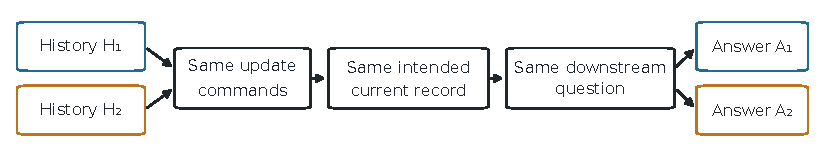
\includegraphics[width=\linewidth]{matched_history_design.pdf}
\caption{\textbf{Matched histories.} Different starting histories receive identical update commands and reach the same intended current record. We verify the facts required by a shared downstream question under every history, and both references must answer correctly before a disagreement counts. The schematic illustrates two histories from the eight-history construction used in the controlled matched-history study; only facts required by the shared downstream question are behaviorally verified.}
\label{fig:matched-history-design}
\end{figure}

\section{Context-sensitive relation readout}
\label{sec:reading-relation}

\subsection{Experimental setup}
We use frozen Llama-3.1-8B-Instruct (32 layers) and Gemma-2-9B-it (42 layers). At each decoder layer, we extract the residual-stream activation at the final prompt token before candidate scoring. The model selects between neutral answer symbols whose mapping to \emph{Supports} and \emph{Opposes} is reversed deterministically across items.

A checkerboard crosses two situations with two considerations, with every row and column represented once under each label. For standardized scores $\tilde{s}_{ij}$, its interaction is
\[
I_b=\tilde{s}_{11}-\tilde{s}_{12}-\tilde{s}_{21}+\tilde{s}_{22}.
\]
Any scorer additive in situation and consideration has zero interaction. We compare a difference-in-means direction and an $L_2$-regularized logistic probe with a text-only classifier over frozen MiniLM embeddings. Readouts are fitted on 1,500 items; 300 separate items select the layer; 500 items (125 checkerboards) form the held-out evaluation. A permutation control assesses the fitting pipeline, and a factual True/False task checks whether it recovers a relation with known truth values. The development data, layer selection, and controls are detailed in Appendix~\ref{app:relation-signal}.

\subsection{Results}
\label{sec:reading-relation-results}
Both models show positive held-out checkerboard interactions for activation readouts (Figure~\ref{fig:construct-validity}). Difference-in-means interactions are 1.647 for Llama and 2.322 for Gemma; logistic-probe interactions are 2.084 and 2.150. The text-only interaction is 0.284 in each model. The comparator uses frozen Sentence-BERT embeddings~\citep{reimers2019sentencebert}. The tested situation-only, consideration-only, and additive controls cancel, and the factual positive control passes. The result supports a linearly accessible context-sensitive signal beyond these controls. It does not show that later behavior causally uses this signal.

\begin{figure}[t]
\centering
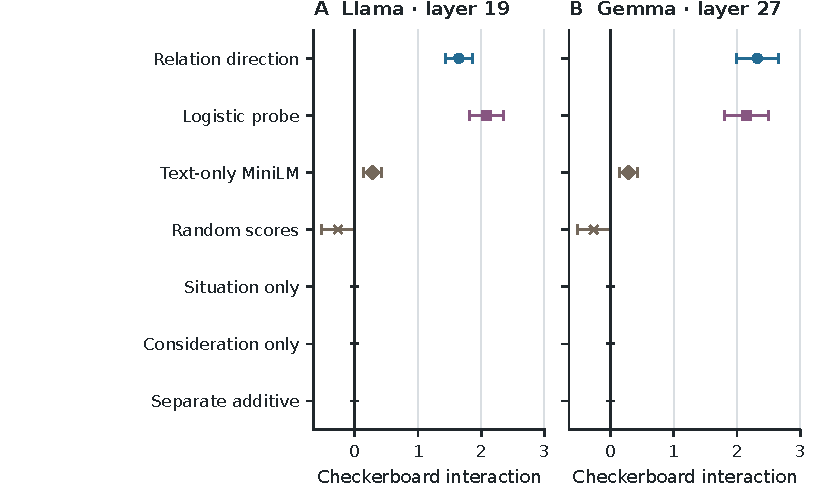
\includegraphics[width=.94\linewidth]{construct_validity.pdf}
\caption{\textbf{Held-out relation interactions.} Standardized checkerboard interaction for activation readouts and controls in Llama and Gemma. Error bars are 95\% dyadic-robust intervals where retained; open markers indicate a point estimate without a retained interval. These are development measurements.}
\label{fig:construct-validity}
\end{figure}

\section{Direct-answer intervention and consequence recovery}
\label{sec:changing-direct-answer}

\subsection{Experimental setup}
Each of 192 synthetic contexts describes four person--proposal stances. A base and counterfactual context differ in one focal stance. Two wordings are used, with 96 contexts reserved for final evaluation. Six binary questions are asked: Q1 directly tests the focal relation; Q2--Q4 test related formulations; Q5--Q6 test unaffected relations. The answer margin is $\log P(\text{ENTAILED})-\log P(\text{NOT\_ENTAILED})$.

The conceptual comparison is between changing one relation feature and changing the complete representation produced by rewriting that relation. At the final prompt token after Gemma layer 27, relation steering adds $\alpha u$ to the base activation, where $u$ is a frozen relation direction. Whole-activation interpolation moves the base activation toward the counterfactual activation, and full replacement uses that counterfactual activation directly:
\[
h_{\mathrm{base}}\mapsto h_{\mathrm{base}}+f(h_{\mathrm{cf}}-h_{\mathrm{base}}).
\]
Steering and interpolation strengths are calibrated using Q1 alone to produce 75\% of its natural margin change, then frozen for Q2--Q6 and the second wording.

For the five non-calibration questions, let $N$ be the margin-change vector produced by rewriting the relation in text and $I$ the vector produced by an intervention. Recovery is $R=1-D(I,N)^2/D(0,N)^2$, where $D$ weights focal consequences and unaffected controls equally. The prespecified rules require the natural counterfactual to pass answer, consequence, control, and wording checks, and require each tuned intervention to meet a full-dose rule (counterfactual answer ahead by at least 1 nat) in at least 90\% of held-out contexts. The Gemma natural counterfactual passes, but both tuned arms miss the full-dose rule: relation steering meets it in 80/96 contexts and whole-state interpolation in 81/96. We therefore report this comparison descriptively. Full details and the other unsuccessful qualification arms are in Appendix~\ref{app:direct-intervention}.

\subsection{Results}
\label{sec:changing-direct-answer-results}
In this descriptive Gemma comparison, relation steering matches the calibrated Q1 target on average but does not recover the natural downstream pattern (Figure~\ref{fig:consequence-qualification}). Its recovery is approximately $-0.85$, compared with $0.914$ for whole-state interpolation and $0.981$ for full replacement. Changing the direct answer and recovering the other consequences of a relation change can therefore come apart. Because neither tuned arm meets the prespecified 90\% full-dose criterion, this contrast is qualification-limited evidence rather than a confirmatory test, and it does not establish that relation steering generally fails in other settings.

\begin{figure}[t]
\centering
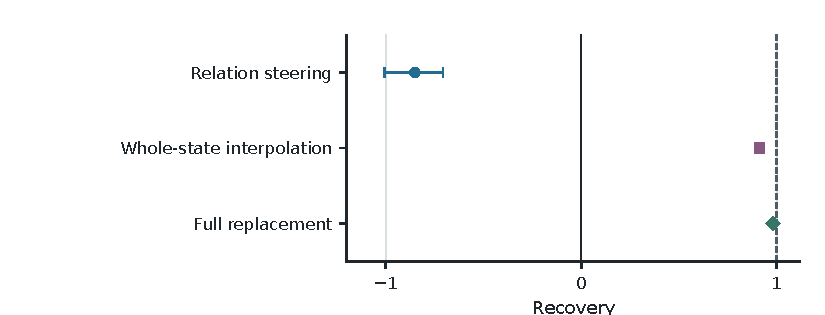
\includegraphics[width=.80\linewidth]{consequence_qualification.pdf}
\caption{\textbf{Consequence recovery after a direct-answer intervention.} Recovery compares the five non-calibration answer-margin changes with the natural textual counterfactual. Steering and interpolation target the same Q1 margin; full replacement is an untuned reference. Intervals are 95\% context-bootstrap intervals. Both tuned arms miss the prespecified 90\% full-dose criterion (80/96 and 81/96 contexts), so the comparison is descriptive (Appendix~\ref{app:direct-intervention}).}
\label{fig:consequence-qualification}
\end{figure}

\section{Matched-history evaluation}
\label{sec:matched-histories}

\subsection{Experimental setup}
A case contains a record of four to six fictional meeting members' stances on two proposals and selects three stances for update. Eight starting histories enumerate all assignments to those selected stances; unselected facts are shared. Every history receives the same three commands, which set the selected facts to the same intended final values. A no-op occurs when a selected fact already has that value. The all-correct starting history is a reference condition.

The four update procedures use frozen Gemma-2-9B-it and Qwen3-8B backbones: a constrained learned editor, a consistency-trained learned editor, existing textual correction, and latest-value wording. Each completed update receives the same question battery on a fresh context copy. The battery contains direct questions and nine joint questions under two answer formats. A joint question is \emph{eligible} only if both required facts are read correctly under all eight histories and both the \emph{current-facts-from-the-start reference} and the \emph{already-correct reference} answer correctly. An eligible joint question is a \emph{witness} if valid downstream answers differ across histories.

The primary outcome is the witness count divided by all 18 scheduled joint-question opportunities per case; ineligible opportunities remain in this fixed denominator. Case-level rates are averaged across the 64 shared designs, and the learned-editor seed rates are averaged within case. We bootstrap over cases and use 99.375\% intervals for eight comparisons. The detailed protocol, seed selection, and inference rules are in Appendix~\ref{app:matched-history-details}.

\subsection{Prospective results}
\label{sec:matched-histories-results}
Witness rates range from 2.39\% to 6.34\% of scheduled opportunities across the eight model/procedure combinations (Figure~\ref{fig:matched-history-results}); all multiplicity-adjusted intervals exclude zero. The finding occurs under both textual and learned updates in both backbones. The intervals describe this controlled case-generating procedure, not deployment frequency.

\begin{figure}[t]
\centering
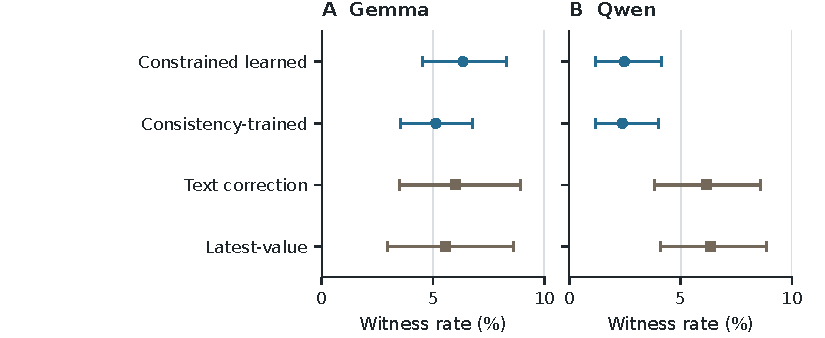
\includegraphics[width=.94\linewidth]{matched_history.pdf}
\caption{\textbf{Prospective matched-history witness rates.} Points show case-averaged witness rates for 64 cases; bars show 99.375\% case-bootstrap intervals. Each case has 18 scheduled joint-question opportunities (1,152 per condition); ineligible opportunities remain in the denominator. Learned seed rates are averaged within case. Eligibility requires correct direct facts under all histories and correct answers from both references; a witness requires valid answers that differ across histories.}
\label{fig:matched-history-results}
\end{figure}

\subsection{Stronger post-hoc controls and fresh confirmation}
We apply controls that match prefix length and changed-fact count and require additional logical questions to be correct. Pooled over both backbones, all four update procedures, and both learned-editor seeds, the complete conjunction leaves 64 of 13,824 coded opportunities across 29 of the original 64 cases (45.3\%); 60 of these opportunities come from learned editors and 4 from textual procedures. The 29-case count measures case recurrence in this pooled post-hoc analysis, not a single-procedure rate, an opportunity-level rate, or deployment prevalence. Decomposition and counting units are in Appendix~\ref{app:matched-history-robustness}.

A fresh 64-case Gemma cohort tests these stronger criteria prospectively using the constrained editor and both stored seeds without refitting. Witnesses remain in 14/64 cases (21.9\%); the case-averaged rate is 0.95\% of prespecified target opportunities (95\% CI: 0.52\%--1.43\%). The case fraction and target-opportunity rate have different denominators. The held-out utility contrast is inconclusive (Appendix Figure~\ref{fig:fresh-confirmation}); we find no established utility advantage.

\subsection{Breadth on reused designs}
Qwen3-32B is evaluated on the same 64 designs with the two textual procedures, using independent full-prefix question passes. Basic witnesses occur in 128/1,152 scheduled opportunities (11.11\%) for existing correction and 123/1,152 (10.68\%) for latest-value wording. This extends model breadth on reused case designs, not independent case replication. Under the strongest two-format criterion, neither procedure has a qualifying witness (0/576 scheduled semantic opportunities); each has a nonempty certified subset. See Appendix~\ref{app:matched-history-robustness}.

\section{Public multi-hop generalization}
\label{sec:mqmh}

We test recurrence on original public multi-hop question phrasings using a frozen 128-subject cohort derived from MQuAKE-CF-3k-v2. Qwen2.5-7B-Instruct and Gemma-2-9B-it are evaluated separately on the same three phrasings per subject (384 scheduled targets per model). This is an explicit-record, in-context counterfactual evaluation, not standard closed-book MQuAKE performance or a parameter-editing study.

Histories H0/H1 contain relevant obsolete records; S0/S1 contain matched obsolete records on an irrelevant entity. Every history receives the same correction block and ends at the same intended current record, while obsolete context remains in the prompt. For a target to pass the common guard, every required current-path fact must be correct under all four histories, and both C (clean current record from the start) and C+ (already-correct record receiving the same no-op corrections) must answer the original question correctly. Fact questions are independent; their answers are not supplied to the multi-hop question. A guarded target qualifies when two histories yield distinct valid entity answers and exactly one is correct.

\begin{table}[!htbp]
\caption{\textbf{MQuAKE-derived public multi-hop results.} Qualified counts use all 384 scheduled targets per model, including failed common guards. The relevance contrast is the common-guard-weighted H0/H1 minus S0/S1 target-error difference over those 384 targets; invalid outputs count as errors. Strong long-chain counts use the 195 scheduled three- and four-hop targets and require a correct independent remaining-chain control under all four histories. Brackets show 98.75\% subject-clustered intervals for the first two measures (Appendix~\ref{app:public-data-details}).}
\label{tab:mqmh}
\centering
\small
\begin{tabular}{lrrr}
\toprule
Model & Qualified history dependence & Relevance contrast & Strong long-chain \\
\midrule
Qwen2.5-7B & 94/384 (24.5\%) [17.7, 31.8] & +12.5 pp [8.3, 17.4] & 32/195 \\
Gemma-2-9B & 101/384 (26.3\%) [18.6, 34.4] & +15.6 pp [10.8, 21.0] & 65/195 \\
\bottomrule
\end{tabular}
\end{table}

The relevance contrast is +12.5 percentage points for Qwen and +15.6 for Gemma under this guarded definition; it is not a raw comparison restricted to targets passing the guard. For strong long-chain witnesses, a separate question starts from the current first-hop answer and tests the remaining chain under every history. The counted cases therefore combine correct reports of all required current facts, correct C/C+ references, and independently successful remaining-chain reasoning, yet the answer to the original question can still depend on relevant obsolete history. These controls make simple explanations based only on missed current facts or inability to traverse the remaining chain insufficient for the counted witnesses. The two models share the cohort; these results do not establish cross-model superiority.

In source case 1617, the public J2 question is “What place did the person who founded William Levada's religion work in?” The benchmark stipulates William Levada → Church of Scotland → John Knox → Edinburgh as the current chain, and Catholic Church → Jesus Christ → Galilee as the obsolete chain. These are counterfactual benchmark stipulations, not biographical claims. All required current facts and the independent remaining-chain answer (Edinburgh) are correct under every history for both models; C and C+ also answer Edinburgh. For Qwen, H0 answers Galilee while H1, S0, S1, C, and C+ answer Edinburgh. For Gemma, H1 answers Galilee while H0, S0, S1, C, and C+ answer Edinburgh. The differing history order does not identify a positional mechanism. Appendix~\ref{app:public-data-details} gives the bootstrap, parser, repeat, and secondary RippleEdits details. Residual pretraining exposure is unknown; transfer to parameter editing and deployment prevalence are not established.
\FloatBarrier

\section{Causal follow-ups}
\label{sec:causal-followups}

\subsection{Selected activation crossover}
\paragraph{Experimental setup.} We exchange the first 16 and remaining 26 Gemma activation layers between two histories that disagree on one downstream question, then ask that question. Relevant direct facts are checked after each exchange. \paragraph{Results.} Among six selected cases, the main answer format follows the later-activation source in five; the alternate format is less consistent. A separately matched one-case extension reproduces the pattern in both formats under the stronger controls (Figure~\ref{fig:selected-crossover}). These selected-case interventions show causal influence under the tested exchange, not population prevalence or a unique storage location.

\begin{figure}[tbp]
\centering
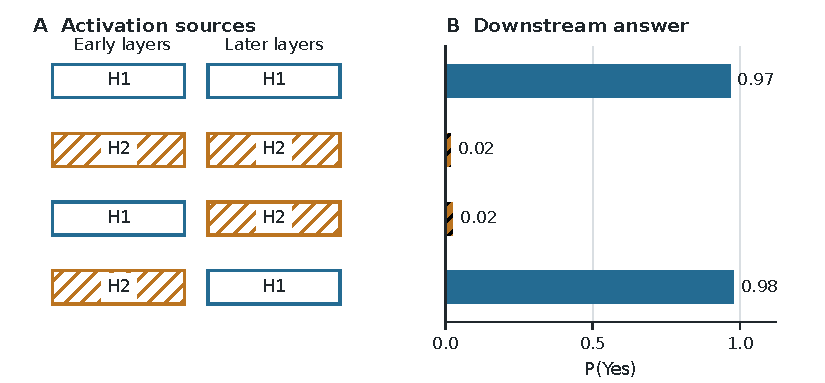
\includegraphics[width=.74\linewidth]{selected_crossover.pdf}
\caption{\textbf{Selected activation crossover.} Each row combines early layers from one history with later layers from the other; downstream answer probabilities change with the later source. Direct-fact checks remain correct. The example was selected for a history effect; the six-case summary and two-format extension are reported in the text and Appendix~\ref{app:causal-details}.}
\label{fig:selected-crossover}
\end{figure}

\subsection{Question-blind refresh}
\paragraph{Experimental setup.} A fixed refresh replaces Gemma cached attention values at layers 16--23 with those from a full-current-record reference before the downstream question is known. \paragraph{Results.} It repairs 36/83 qualifying failures across 28 designs, compared with 2/83 for a later-layer comparison. The prespecified threshold of repairing at least half of qualifying failures is not met. Across all scheduled joint responses, targeted refresh corrects 944 errors and introduces 347; total joint errors fall from 3,490 to 2,893. The reference itself has 2,000 errors. Refresh therefore provides partial repair with collateral errors, not a general update solution (Appendix Figure~\ref{fig:repair-benefit-damage}).

\section{Related work}
\label{sec:related-work}
Standard MQuAKE~\citep{zhong2023mquake} evaluates downstream answers after knowledge edits; our MQuAKE-derived study instead supplies explicit counterfactual records in context, matches histories to a shared intended record, and gates history-dependent answers on current-fact and clean-reference checks. It is not a closed-book benchmark result or a parameter-editing evaluation. RippleEdits~\citep{cohen2024ripple} and analyses of multi-hop shortcuts~\citep{ju2024shortcuts} likewise show that correct atomic facts need not compose correctly. Work on editing pitfalls~\citep{li2024pitfalls} and surface compliance~\citep{gu2026surface} further motivates checking behavior beyond an edit's immediate target.

Linear probes and difference-in-means directions test which distinctions are accessible in activations; probing methodology cautions that accessibility alone does not establish causal use~\citep{burns2023discovering,elazar2021amnesic}. Representation engineering and inference-time intervention use activation directions to alter outputs~\citep{li2023inference,turner2023activation,zou2023representation}. Our contribution is to separate direct-answer change from recovery of the natural multi-question consequence pattern, then test history dependence after updates through matched histories.

State-based evaluation asks whether different trajectories that reach a common state still yield different predictions~\citep{vafa2024worldmodel}. Model editing research also studies parameter updates and the localization of factual associations~\citep{mitchell2022mend,meng2022rome,meng2023memit}. We adapt the state-sufficiency question to language-model updates: histories receive identical commands and reach the same intended current record, while the question-required facts are read correctly under every history and both references answer correctly. We do not require identical internal states. The activation crossover and refresh test whether this dependence is manipulable under specific interventions. Appendix~\ref{app:related-work-background} discusses these connections and their boundaries in more detail.

\section{Conclusion}
Direct correctness is a necessary but incomplete check of an update. In the controlled matched-history study, earlier histories can still predict a downstream answer after question-required facts and both references pass their checks. This pattern also recurs on MQuAKE-derived public multi-hop phrasings in two model families: some counted long-chain witnesses report the required current facts, answer clean/no-op references correctly, and independently traverse the remaining chain, yet answer the original question differently across relevant histories. Linear readout, the qualification-limited direct-intervention comparison, and selected causal follow-ups address distinct aspects of representation and behavior; none identifies a unique mechanism. These results motivate evaluating whether an update governs the downstream behavior it is meant to change. Appendix~\ref{app:limitations} discusses scope and limitations.

\subsection*{Ethics statement}
We treat ValuePrism labels as dataset annotations and the synthetic meeting records as fictional. The experiments do not measure human moral judgment or support claims about population values.

\subsection*{AI use statement}
Generative AI tools assisted substantially with manuscript drafting, restructuring, technical and language editing, reference discovery and checking, revisions to figure sources and plotting code, and checking and describing retained results. During manuscript revision, AI tools did not generate new experimental measurements, run pretrained-model inference, or retrain models. AI-assisted text, figures, and statistics were checked against the retained evidence and reconstruction code; the authors remain responsible for the final content. The available records do not establish whether AI was used for experiment design, methodology, implementation beyond the documented revisions, synthetic-data generation, hypothesis formulation, or other research-activity categories. Authors must verify those categories and ensure the OpenReview disclosure matches this statement.

\subsection*{Reproducibility statement}
The accompanying anonymous supplementary code package contains retained measurements, manifests, source code, figure-generation code, and CPU analyses that reconstruct supported statistics and gates. Appendix sections document each study's settings and reproduction boundaries. Fresh pretrained execution and complete retraining are not verified by the supplied artifacts; no anonymous hosting URL is claimed here.

\bibliography{references}
\bibliographystyle{iclr2027_conference}

\appendix

% ============================================================
% A. RELATION SIGNAL
% ============================================================

\section{Relation-Signal Details}
\label{app:relation-signal}

\subsection{Data splits and layer selection}

The relation-signal experiments use Llama-3.1-8B-Instruct and
Gemma-2-9B-it with frozen weights. We extract the residual-stream activation
at the final prompt token before the model scores the answer candidates.

For each model, 1,500 ValuePrism rows are used to fit the readouts.
A separate set of 300 rows, forming 75 checkerboards, is used for layer
selection. Final evaluation uses 500 rows forming 125 held-out checkerboards.
The evaluation boards play no role in fitting the readouts or choosing the
layer.

\begin{table}[htbp]
\caption{Relation-signal splits and selected layers.
Readouts are fit on the training rows, layers are chosen on a separate
selection split, and the reported checkerboard results use held-out evaluation
boards.}
\label{tab:relation-splits}

\centering
\small
\begin{tabular}{lrrrr}
\toprule
Model & Train rows & Selection rows & Eval. rows & Selected layer \\
\midrule
Llama-3.1-8B-Instruct & 1500 & 300 & 500 & 19 \\
Gemma-2-9B-it & 1500 & 300 & 500 & 27 \\
\bottomrule
\end{tabular}


\end{table}

The primary readout is a difference-in-means direction. For each model and
layer, we subtract the mean activation of Opposes examples from the mean
activation of Supports examples and normalize the result to unit length.
An example is scored by projecting its activation onto this direction.

We also fit an L2-regularized logistic probe to the same activations. The
selected layer maximizes discrimination within situations and within
considerations on the selection split. This gives layer 19 for Llama and
layer 27 for Gemma.

\subsection{Checkerboard interaction}

Each checkerboard contains two situations and two considerations. Every
situation and every consideration appears once under Supports and once under
Opposes. For standardized scores $\tilde{s}_{ij}$, the interaction is

\[
I_b
=
\tilde{s}_{11}
-
\tilde{s}_{12}
-
\tilde{s}_{21}
+
\tilde{s}_{22}.
\]

Any score of the additive form
$f(s,c)=a(s)+b(c)$ has $I_b=0$. The checkerboard statistic therefore removes
fixed situation effects, fixed consideration effects, and their additive
combination. Positive interaction requires the score to depend on how the
situation and consideration are paired.

The difference-in-means direction reaches $I_b=1.647$ in Llama and
$I_b=2.322$ in Gemma. The logistic probe reaches $2.084$ and $2.150$,
respectively.

\subsection{Text-only comparison}

The text-only comparison asks how much of the same relation can be predicted
without access to model activations. We embed the situation and consideration
with frozen all-MiniLM-L6-v2 embeddings. The classifier receives the two
embeddings together with their elementwise product and absolute difference,
then fits logistic regression using the same training split.

The text-only classifier is evaluated on the same held-out checkerboards as
the activation readouts. Its checkerboard interaction is approximately
$0.284$ in both model experiments. This provides a comparison for relation
structure available directly from the input wording.

\subsection{Permutation control}

The permutation control tests whether the fitting pipeline can produce a
large checkerboard interaction after the support/opposition orientation is
randomized. Each training situation independently keeps or reverses all of its
labels. The training rows and situation groupings remain fixed. The readouts
are refit for every permutation and evaluated on the unchanged held-out
checkerboards.

The later Llama analysis uses 10,000 permutations. The
difference-in-means direction gives a one-sided empirical
$p=0.0132$, while the logistic probe gives $p=0.0001$. The corresponding
two-sided sensitivity value for the difference-in-means direction is
$p=0.0245$.

The retained Gemma permutation analysis uses 200 draws. The
difference-in-means direction gives $p=0.0149$, and the logistic probe reaches
the resolution floor of $1/201$.

\subsection{Factual positive control}

A separate factual task checks whether the same extraction and fitting
pipeline can recover a semantic distinction with known ground truth. The task
uses factual True/False labels but presents them through neutral answer
symbols whose meanings are reversed across examples. A separate prompt
condition also changes the answer symbols.

The factual control contains 748 proposition groups. Within the primary answer
scheme, 1,796 records fit the directions, 600 select the layer, and 596 remain
held out for final evaluation.

\begin{table}[htbp]
\caption{Factual positive control.
The same direction-fitting pipeline separates held-out factual classes under
neutral and reversed answer mappings in both model families.}
\label{tab:factual-control}

\centering
\small
\begin{tabular}{lrr}
\toprule
Model & Selected layer & Held-out separation $T$ \\
\midrule
Llama-3.1-8B-Instruct & 14 & 1.924 \\
Gemma-2-9B-it & 25 & 1.944 \\
\bottomrule
\end{tabular}


\end{table}

For Llama, none of 1,000 group-preserving null runs reaches the observed
statistic. The add-one permutation value is therefore $1/1001$. Gemma shows
the same qualitative positive-control result. These controls establish that
the readout pipeline can recover a known semantic distinction across changed
answer mappings.


% ============================================================
% B. DIRECT INTERVENTION
% ============================================================

\section{Direct-Intervention Details}
\label{app:direct-intervention}

\subsection{Contexts and questions}

The intervention experiment uses 192 synthetic contexts. Each context names
two people and two proposals and states whether each person supports or
opposes each proposal. One of the four person--proposal relations is the
focal stance. The base and counterfactual contexts differ only in this
relation.

We use 32 contexts to select the prompt protocol, 64 for fitting and
calibration, and 96 as held-out final contexts. Each context is rendered in
two alternative wordings.

Every context receives six binary questions. Q1 directly asks about the
counterfactual focal relation and is the only question used to select
intervention strength. Q2 asks the complementary claim. Q3 and Q4 rephrase
the same focal relation. Q5 and Q6 ask about unaffected relations and serve
as stability controls.

For each question, the answer margin is

\[
m
=
\log P(\text{ENTAILED})
-
\log P(\text{NOT\_ENTAILED}).
\]

\subsection{Interventions}

All interventions act on the residual stream after layer 27 of Gemma at the
final prompt token. Let $h_{\mathrm{base}}$ denote the activation under the
base context and $h_{\mathrm{cf}}$ the activation under the counterfactual
context for the same question.

Relation steering changes only the component along the frozen
support/opposition direction $u$:

\[
h_{\mathrm{base}}
\mapsto
h_{\mathrm{base}}+\alpha u.
\]

The sign of $\alpha$ points toward the counterfactual relation.

Whole-activation interpolation instead moves the complete activation toward
the activation produced by rewriting the relation in text:

\[
h_{\mathrm{base}}
\mapsto
h_{\mathrm{base}}
+
f\left(h_{\mathrm{cf}}-h_{\mathrm{base}}\right).
\]

Full replacement substitutes $h_{\mathrm{cf}}$ for $h_{\mathrm{base}}$.
It serves as a reference for the activation change produced by the complete
textual counterfactual.

\subsection{Calibration}

The steering coefficient $\alpha$ and interpolation fraction $f$ are selected
using Q1 alone. The target is 75\% of the natural margin change between the
base and counterfactual contexts. Once selected, the intervention strength is
frozen.

Q2--Q6 never contribute to calibration. They are evaluated only after the
strength has been fixed. The same intervention strength is also used for the
second wording.

\subsection{Consequence-recovery score}

Changing the focal relation in text produces a vector of margin changes on
Q2--Q6. We call this the natural signature $N$. An intervention produces its
own vector $I$ on the same questions.

Each question dimension is standardized using a robust scale estimated from
the fitting contexts. The distance gives equal total weight to Q2--Q4 and to
the two stability controls Q5--Q6.

Counterfactual signature recovery is

\[
\mathrm{CSR}
=
1-
\frac{D(I,N)^2}
     {D(0,N)^2}.
\]

A score of 1 reproduces the natural counterfactual signature. A score of 0
leaves the held-out questions at their base behavior. Negative values move
farther from the natural signature than the unchanged base state.

Uncertainty intervals use 10,000 bootstrap resamples of the held-out
contexts while preserving paired measurements within each context.

\subsection{Qualification}

The prespecified full-dose rule requires each tuned intervention to make the
counterfactual answer the higher-probability choice with a margin of at least
1 nat in at least 90\% of the held-out contexts. Neither tuned arm meets it:
relation steering satisfies the rule in 80/96 contexts and whole-state
interpolation in 81/96, although both match the calibrated Q1 target on
average. Section~\ref{sec:changing-direct-answer} therefore reports the
recovery comparison descriptively rather than as a qualified confirmatory
test. Full replacement is an untuned reference and is not calibrated.

The natural counterfactual context must also answer accurately, produce the
expected changes on focal questions, remain stable on unaffected questions,
and agree across the two wordings. Gemma passes these qualification checks.
The corresponding Llama reference fails the frozen qualification criteria and
is excluded from the consequence-recovery comparison.

A support/opposition direction refit directly in the intervention prompt
format also fails qualification. The steering experiment therefore uses the
original frozen relation direction from Section~\ref{sec:reading-relation}.


% ============================================================
% C. MATCHED HISTORIES
% ============================================================

\section{Matched-History Experimental Details}
\label{app:matched-history-details}

\subsection{Records and starting histories}

Each record describes four to six fictional meeting members and two
proposals. A sentence records each person's stance toward a proposal.

A case selects three stances for update. The eight starting histories cover
all $2^3$ assignments to these three stances. Every other fact is held fixed.
All eight histories then receive the same three update commands, which set
the selected stances to the same intended final values.

If a selected stance already has the requested final value, its update is a
no-op. The history in which all three selected stances already equal their
final values supplies the already-correct reference condition.

\subsection{Questions and answer formats}

Each updated record receives a fixed question battery. Direct questions ask
about a single stance. Joint questions combine two stances. The joint
questions ask whether two members take the same side, whether both support a
proposal, or whether either supports it.

The full battery contains 34 questions. The primary matched-history analysis
uses 18 joint opportunities per case: nine semantic joint questions under two
answer formats.

One answer format uses literal \emph{No}/\emph{Yes}. The second uses the
symbols A/B with a fixed mapping to no and yes. The predicted answer is the
candidate with the larger answer-token log-probability.

\subsection{Backbones}

The primary matched-history study uses Gemma-2-9B-it and Qwen3-8B. Gemma has
42 decoder layers. Qwen3-8B has 36. Both backbones remain frozen and run in
bfloat16. Qwen uses its non-thinking chat configuration.

\subsection{Learned update procedures}

The learned editors alter the stored representation of the record while
leaving the visible text unchanged. The update module receives the record
prefix, the token span corresponding to the stance being changed, and the
requested new value. It edits the residual-stream representation at one
decoder layer. The remaining decoder layers are then recomputed from the
edited prefix.

The Gemma editor intervenes at layer 15. The Qwen editor intervenes at
layer 13.

The constrained editor limits the update to a fixed 16-dimensional subspace
chosen to preserve readouts of facts that are not being changed. Training
optimizes the likelihood of the requested new answer.

The consistency-trained editor removes the preservation-subspace restriction
and adds a symmetric KL consistency term that discourages unintended changes
to the two-label answer distribution.

Both learned update procedures are trained for one epoch with the backbone
frozen. Each procedure is evaluated using two stored training seeds.

\subsection{Textual update procedures}

The textual procedures leave model weights and activations untouched and
modify the record itself.

\emph{Existing correction} appends one correction sentence for each command
in command order. A correction has the form

\begin{quote}
Correction: the record for Ari on the Library proposal is updated.
Ari is now opposed to the Library proposal.
\end{quote}

\emph{Latest-value wording} uses the same correction content but orders the
corrections by the corresponding location in the original record.

No update procedure receives the downstream question before all updates are
complete. Every question is evaluated from a fresh copy of the resulting
context.

\subsection{References and eligibility}

Two references determine whether a downstream disagreement is interpretable.

The current-facts-from-the-start reference presents the final record directly.
It therefore tests whether the model can answer the downstream question when
no conflicting earlier values are present.

The already-correct reference starts from the history where the selected
stances already hold their target values and applies the same update
procedure. It tests the update machinery in a condition where the requested
facts require no semantic change.

A joint question is eligible only when both required direct facts are read
correctly under all eight histories and both references answer the joint
question correctly.

An eligible joint question is a witness when its valid answer differs across
histories.

\subsection{Aggregation and uncertainty}

The primary study uses 64 cases for each backbone. Each case contributes 18
scheduled joint opportunities. Ineligible opportunities remain in the
denominator.

For learned editors, the two training-seed rates are averaged within each
case before aggregation. Textual procedures contribute one measurement per
case.

Uncertainty is computed by resampling the 64 cases with replacement
10,000 times. Each of the eight model--procedure combinations uses a
99.375\% interval. The eight simultaneous intervals therefore maintain a
5\% overall error rate.


% ============================================================
% D. ROBUSTNESS AND BREADTH
% ============================================================

\section{Matched-History Robustness and Breadth}
\label{app:matched-history-robustness}

\subsection{Matched-history robustness analysis}

The first robustness analysis reuses saved outputs from the prospective
study. It applies two restrictions that were specified after the primary
results were known.

First, the two histories being compared must require the same number of
actual fact changes and must have exactly the same rendered prefix-token
length.

Second, surrounding logical questions must be answered correctly. For a
target pair of stances, the same-pair controls ask the other two Boolean
questions about that pair. For example, a target asking whether two people
take the same side is accompanied by questions asking whether both support
the proposal and whether either supports it.

Cross-pair controls apply all three Boolean question forms to the other
selected stance pairs.

Matching on changed-fact count and prefix length retains 430 of the 653
original witnesses. Requiring both the same-pair and cross-pair logical
controls leaves 64 coded opportunities across 29 of the 64 original cases.
These counts pool both backbones, all four update procedures, and both
learned-editor seeds, out of 13,824 coded opportunities; 60 of the 64
surviving opportunities come from the two learned editors and 4 from the two
textual procedures (one per backbone and procedure). The 29-case figure is
therefore pooled case-level recurrence, not a per-procedure rate.

\subsection{Fresh prospective confirmation}
\label{app:fresh-confirmation}

The stronger controls were then tested on a fresh cohort of 64 Gemma cases.
The experiment uses the same record construction, downstream questions, and
constrained learned editor as the primary study. Both stored training seeds
are evaluated without refitting.

The history-matching requirement and logical controls were fixed before
model inference on the new cases. History-dependent answers recur in 14 of
64 cases. Across all scheduled target opportunities, the mean witness rate is
0.95\%, with a 95\% interval of 0.52--1.43\%.

A separate utility analysis asks whether filtering updates with the stronger
history criterion reduces error on held-out questions. At 50\% case
retention, the paired error contrast is $-1.74$ percentage points with a
95\% interval of $[-3.53,\,0.65]$. The recurrence result therefore survives
prospective testing, while the update-selection comparison remains
inconclusive.

\begin{figure}[htbp]
    \centering
    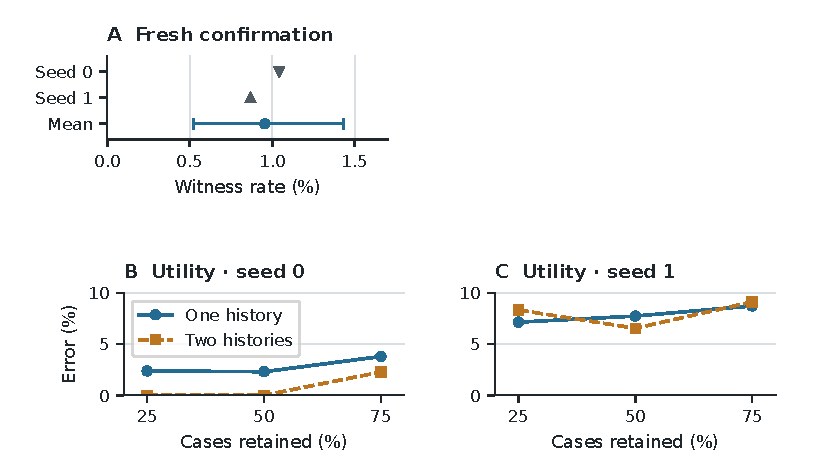
\includegraphics[width=.82\linewidth]{fresh_confirmation_utility.pdf}
    \caption{
    \textbf{Fresh prospective confirmation and utility comparison.}
    The stronger matching and logical controls are fixed before inference on
    a new 64-case Gemma cohort. History dependence recurs in 14 cases.
    The held-out-error comparison has an interval spanning zero.
    }
    \label{fig:fresh-confirmation}
\end{figure}

\subsection{Qwen3-32B breadth}

We also evaluate Qwen3-32B on the same 64 case designs using the two textual
update procedures. These are new model measurements on existing cases rather
than a fresh sample of cases.

Every complete prompt is processed independently with thinking disabled.
No key/value cache is reused across prompts.

\begin{table}[htbp]
\caption{Qwen3-32B textual matched-history results.
The same fixed cases and qualification rules are evaluated with full-prompt
recomputation on the larger checkpoint.}
\label{tab:qwen32}

\centering
\small
\begin{tabular}{lrrr}
\toprule
Procedure & Witnesses & Rate & Cases with witness \\
\midrule
Existing correction & 128/1152 & 11.11\% & 43/64 \\
Latest-value wording & 123/1152 & 10.68\% & 49/64 \\
\bottomrule
\end{tabular}


\end{table}

The strongest cross-format criterion requires the same logically controlled
disagreement to survive both answer formats. Neither textual procedure
produces a witness under that criterion. Each procedure has 80 fully
logically certified semantic opportunities across nine cases before the
cross-format disagreement requirement is applied.


% ============================================================
% E. CAUSAL FOLLOW-UPS
% ============================================================

\section{Causal Follow-Up Details}
\label{app:causal-details}

\subsection{Causal crossover}

The crossover experiment starts from Gemma histories that already disagree
on the same downstream question after a learned update.

For each selected pair, we construct hybrid computations using the first
16 decoder layers from one history and the remaining 26 layers from the
other. Both directions are tested. Model weights remain fixed. The
downstream question is introduced only after the hybrid state has been
constructed.

The relevant direct facts are checked separately after the crossover. The
main answer format produces five cases where the downstream answer follows
the history supplying the later activations and one mixed case. Results in
the second answer format are less consistent.

A separate matched case also satisfies the stronger history-matching and
logical controls. In that case the crossover repeats under both answer
formats while the required direct facts remain correct.

The crossover therefore tests a causal property of the stored computation:
changing which history supplies the later activations can change the
downstream answer while the relevant factual readouts remain stable.

\subsection{Question-blind refresh}
\label{app:question-blind-refresh}

The refresh experiment asks whether some history-dependent failures can be
corrected before the downstream question is known.

For each Gemma record, a reference state is built from the complete current
record under the same learned update. Before any downstream question is
opened, cached attention values at aligned trailing positions are copied from
this reference into the history-dependent state.

The targeted refresh replaces values from layers 16--23. A comparison
condition performs the same operation using layers 24--31. Keys, model
weights, and the original prompt remain fixed. Every downstream question is
evaluated from an independent copy of the refreshed state.

A repair is counted when the previously failing target becomes correct across
all histories while the required direct and logical-control answers remain
correct.

The prospective population contains 256 cases evaluated under both stored
training seeds. There are 83 qualifying target/format/seed failures in the
baseline cohort. The targeted refresh repairs 36 of these failures, spanning
28 cases. The comparison refresh repairs 2 of 83.

The prespecified strong-repair criterion requires at least half of qualifying
failures to be repaired. The targeted intervention reaches 43.4\%.

The intervention also creates new errors. The complete error accounting is
shown in Figure~\ref{fig:repair-benefit-damage}. Across the full evaluation,
joint errors fall from 3,490 to 2,893 after the targeted refresh.

\begin{figure}[htbp]
    \centering
    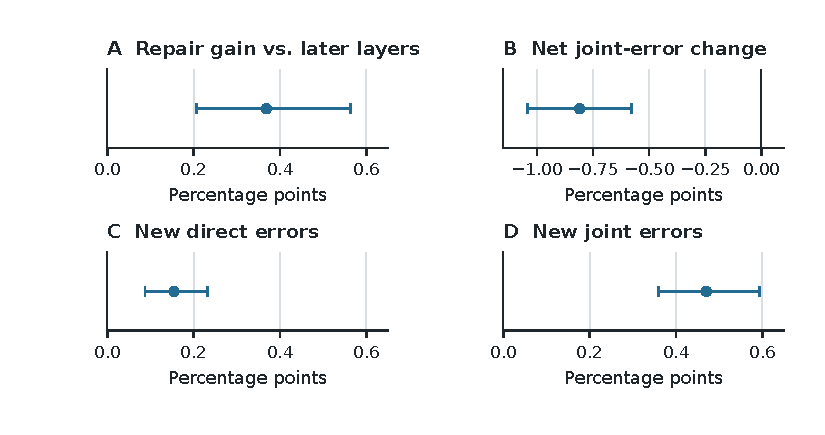
\includegraphics[width=.82\linewidth]{repair_benefit_damage.pdf}
    \caption{
    \textbf{Question-blind refresh.}
    Cached attention values are replaced before the downstream question using
    a complete-current-record reference. Points show estimates with 98.75\%
    intervals. (A)~Repaired qualifying failures, targeted refresh (layers
    16--23) minus the later-layer comparison (layers 24--31), per 9,216
    scheduled target observations. (B)~Change in joint errors, targeted
    refresh minus no refresh, per 73,728 joint responses. (C, D)~New direct
    errors (per 49,152 direct responses) and new joint errors (per 73,728)
    introduced by the targeted refresh.
    }
    \label{fig:repair-benefit-damage}
\end{figure}


% ============================================================
% F. PUBLIC DATA
% ============================================================

\section{Public Multi-Hop and Public-Data Extension Details}
\label{app:public-data-details}

\subsection{MQuAKE-derived public multi-hop study}

The saved-response reconstruction uses the same frozen cohort for both models: 128 subjects and three original public target phrasings per subject. The 384 scheduled targets are the denominator for each model, including failed guards. Required current facts are queried independently and are not fed into the target question. The common guard requires every required fact to be correct under H0, H1, S0, and S1, plus correct target answers from C and C+.

The relevance contrast is the per-target common-guard indicator times the mean H0/H1 target error minus the mean S0/S1 target error, averaged over all 384 scheduled targets. Invalid outputs count as errors; failed guards contribute zero. The long-chain subset contains 195 three- and four-hop targets per model. Strong long-chain qualification further requires the independently prompted remaining-chain question to be correct under all four histories.

Intervals use 10,000 subject-clustered bootstrap draws, resampling each subject with all three target phrasings together, seed 20260923, and 98.75\% coverage. The resulting intervals are 17.7--31.8\% (Qwen) and 18.6--34.4\% (Gemma) for qualified history dependence, and +8.3 to +17.4 and +10.8 to +21.0 percentage points for the relevance contrast. They are approximate constructed-sample intervals; relation families and shared intermediates may remain dependent across subjects. Under the strict canonical-label parser, qualified counts are 87/384 (Qwen) and 98/384 (Gemma), and strong long-chain counts are 29/195 and 63/195. Cross-phrasing long-chain subjects number 11 and 21, respectively. Each model has 12/12 semantically stable complete-case fresh-process repeats, including case 1617. Repeat selections comprise eight preselected and four fixed-order positive cases; they do not expand the cohort or repeat every positive. No new inference was performed for this reconstruction. Residual pretraining exposure is unknown, and this shared-cohort study establishes neither deployment prevalence, parameter-editing transfer, nor cross-model superiority.

\subsection{RippleEdits-derived secondary extension}

The public-data experiment uses RippleEdits-derived update questions with
Qwen2.5-7B-Instruct. The evaluated model revision is
\texttt{a09a35458c702b33eeacc393d103063234e8bc28}. Model weights remain fixed.

Each input first supplies an obsolete value and later states an authoritative
replacement. The model is then asked a downstream question whose answer
depends on the replacement.

A candidate counts only when the model first reports the current value
correctly. A clean reference containing the current information without the
obsolete history must also answer the downstream question correctly. These
conditions separate the history-dependent failure from inability to read the
new value or inability to answer the question from the current information.

The final evaluation contains 98 downstream questions spanning 34
RippleEdits-derived benchmark cases. Answers are scored with a parser fixed before final inference. A
second, more conservative parser is retained as a sensitivity analysis.

\begin{table}[htbp]
\caption{RippleEdits-derived public-data extension.
Each retained case reports the replacement value correctly and passes the
clean current-only reference. The downstream answer nevertheless follows the
superseded value from the earlier history.}
\label{tab:ripple-extension}

\centering
\small
\begin{tabular}{lrr}
\toprule
Scoring rule & History-dependent cases & Questions evaluated \\
\midrule
Primary parser & 3 & 98 \\
Alternative parser & 2 & 98 \\
\bottomrule
\end{tabular}


\end{table}

In each of the three primary cases, the incorrect downstream answer is the
value that the authoritative update replaced. Two cases remain under the
alternative parser.

The experiment evaluates explicitly retained in-context history. It does not
apply a parametric model editor. Each query uses a fresh generation cache, so
the result does not depend on a persistent cache carried between independent
questions.


\section{Related-Work Background}
\label{app:related-work-background}

\paragraph{Probing and causal interpretation.} Linear probes provide a controlled test of whether information is accessible in a representation, but probe performance depends on the representation, data, and readout class. Difference-in-means directions and supervised probes have been used to expose latent distinctions~\citep{burns2023discovering}; amnesic probing shows why decodability should be separated from the effect of removing or manipulating the information~\citep{elazar2021amnesic}. Our checkerboard balances two additive feature families and includes textual and factual controls. It supports a claim about linear accessibility within this construction, not a claim that the measured direction is the model's unique or behaviorally operative representation.

\paragraph{Representation engineering and interventions.} Activation steering changes model outputs by adding or extracting directions, while inference-time interventions target selected internal representations~\citep{li2023inference,turner2023activation,zou2023representation}. Such interventions make a distinction experimentally manipulable, but a change to a target response need not reproduce every consequence of a natural textual change. We operationalize this gap with a direct calibration question and a separate, prespecified set of consequence and control questions. The comparison is qualification-limited and descriptive under the gates detailed in Appendix~\ref{app:direct-intervention}.

\paragraph{Knowledge editing and downstream consistency.} Parameter-editing methods such as MEND, ROME, and MEMIT modify model parameters to update factual associations~\citep{mitchell2022mend,meng2022rome,meng2023memit}. Standard MQuAKE and RippleEdits evaluate downstream behavior after knowledge edits and show that target success need not guarantee consistent dependent answers~\citep{zhong2023mquake,cohen2024ripple,ju2024shortcuts}. Our MQuAKE-derived evaluation instead presents explicit counterfactual records in context, matches histories to one intended current record, and tests history dependence only after question-required current facts and clean/no-op references pass. It is neither standard closed-book MQuAKE performance nor parameter-editing evidence.

\paragraph{Path dependence and state sufficiency.} Evaluations of implicit world models ask whether histories leading to equivalent states support consistent predictions~\citep{vafa2024worldmodel}. Surface-compliance analyses also motivate distinguishing agreement with a correction from durable behavioral change~\citep{gu2026surface}. Recent work discusses KV caches as editable and composable computation~\citep{li2026prefill}. Our source-history criterion is behavioral: for each tested question, answers should be invariant to history once its required facts are read correctly under every history and both reference conditions answer correctly. It does not posit that a language model has a singular explicit state, nor does equality of reported facts imply equality of hidden activations.

\section{Limitations and Scope}
\label{app:limitations}
The central matched-history task uses fictional meeting records and controlled support/opposition judgments. It isolates history dependence when all facts required by each compositional question are read correctly under every history and both references answer correctly, but does not represent the breadth of open-ended natural-language updates or high-stakes deployment. ValuePrism relation readout concerns value-conditioned support/opposition judgments, not moral competence in general.

The MQuAKE-derived public multi-hop study uses the same 128 subjects for both models, with 384 scheduled phrasings per model (including failed guards) and 195 scheduled three- and four-hop phrasings. Its strong-witness controls make simple current-fact and remaining-chain competence explanations insufficient for the counted targets, but do not identify a complete internal mechanism. Residual pretraining exposure is unknown; this shared-cohort result establishes neither cross-model superiority nor transfer to parameter editing.

The primary rates use a fixed set of 64 case designs and 18 scheduled target opportunities per case. Their denominators include ineligible opportunities, and the resulting estimates describe this controlled case-generating procedure. The 29/64 and 14/64 stronger-control counts are case-level recurrence; the 29/64 count pools eight model/procedure combinations. The fresh confirmation is prospective for its cohort but uses the same task family; Qwen3-32B uses reused designs and therefore adds model breadth, not independent case replication. The RippleEdits-derived extension has three qualifying primary-parser questions among 98 scheduled questions from 34 benchmark cases; parser sensitivity reduces that count to two. It shows recurrence, not prevalence.

The activation crossover uses six selected cases, with a stronger two-format extension in one case. These interventions support causal influence under the tested exchange but do not locate where history dependence first arises or establish a complete mechanism. The refresh is population-based within its supplied cohort, but only partly repairs failures, misses its prespecified threshold, and introduces errors. Neither intervention defines a general repair method.

The direct-intervention comparison is descriptive and qualification-limited: relation steering meets the full-dose rule in 80/96 contexts and whole-state interpolation in 81/96, both below the required 90\%; the Llama natural reference and the refit-direction arm fail their own qualification checks. The relation readout is development evidence, and the repository records incomplete artifacts for fully fresh reproduction of some readouts and controls. Across all studies, model-family coverage is limited to the named checkpoints and update procedures. No result establishes a unique storage site, universal path dependence, a prevalence estimate for deployment, or how effects scale to longer histories and more complex tasks.

\end{document}
